\documentclass[article]{jlreq}

\usepackage{graphicx}
\usepackage{amsmath,amssymb,amsthm}
\usepackage{siunitx}
%\usepackage{physics}
\usepackage{bm}

%\renewcommand{\today}{\the\year/\the\month/\the\day}
%\renewcommand{\contentsname}{Contents}

%\renewcommand{\refname}{References}
%\renewcommand{\figurename}{Fig.~}
%\renewcommand{\tablename}{Table~}

\begin{document}
\title{Modulation Anode Voltage Controller}
\author{Shin-ichi YOSHIMOTO}
\maketitle
%%\tableofcontents
%%\clearpage


\section{クライストロンビーム電流制御}

クライストロンへのRF入力を変化させることで、空洞電圧$V_c$を制御する。もし、クライストロン電源の直流入力電力を一定に保つとすると、クライストロンのRF出力が低い時は、コレクタ損失が非常に大きくなる。そこで、消費電力の低減とコレクタの過熱防止のため、クライストロンのビーム電流を必要なRF出力で制御する方式をTRISTAN加速器時代から採用している。図\ref{mod_anode}に本方式のブロック図を示す。クライストロン入力のRF振幅はリニア検波され、関数変換器に入力される。関数変換器は、必要なRF電力を出力するのに十分なビーム電流を与えるために、変調アノード電圧に適した関数を生成する。

この関数は、クライストロン入力がTurn Up Pointで設定された値を超えるまではBiasで設定した一定の制御を出力し、Turn Up Pointを超えるとCoeff.で設定する傾きを持った一次関数で制御電圧はVa Limitで設定した電圧まで増加する。このVa Limitによってアノード電圧がカソード電圧よりも低い電圧になるよう制限している。もう1つはリミットは、コレクタの消費電力をあらかじめ設定した値に制限するものである。図\ref{func_conv}に関数変換器の出力を示す。

このシステムは基本的に開ループであるが、$V_c$フィードバックループの摂動源として作用する。したがって、システムの応答速度は$V_c$ループの応答速度よりはるかに遅くなければならない。この要件は、変調アノード電源として本質的に低速のコッククロフト・ウォルトン回路を使用しているため、自動的に満たされる。このシステムの応答速度は約0.3秒である。このシステムが$V_c$フィードバックループに与えるもう一つの効果は、ループゲインをRFパワーレベルに依存させることである。RFパワーレベルによってクライストロンビーム電流が決まり、それによってクライストロンゲインが決まり、結果的に$V_c$フィードバックループのループゲインが決まる。ループゲインは\qty{5}{\kilo\watt}から\qty{800}{\kilo\watt}のRFパワー範囲で約\qty{15}{\decibel}変化する。

クライストロンのビーム電流は、アノード電圧の$3/2$乗でコントロールされる、$I_b \propto V_a^{3/2}$。 カソード電圧($V_k$)は$\pm\qty{1}{\percent}$で一定であり、コレクターでの損失($P_{cl}$) をあまり大きくない範囲に納めようとするならば、RF出力($P_{rf}$) と相関をもって、ビーム電流 ($P_{dc} = V_k\times I_b$) をコントロールする必要がある。
%
\begin{equation}
    P_{dc} = P_{rf} + P_{cl} \notag
\end{equation}
%
ただし、このことより空胴の加速電圧($V_c$)を一定にするフィードバックループののゲインは、RF出力によって変動するようになる(最小ー最大で約\qty{15}{\decibel}のgainが変化)。ビーム電流のコントロールのブロック図を図\ref{mod_anode}に示す。ここで、アノード電圧のコントロール信号としては、クライストロン入力を検波した信号を用いている。この方法はMRの電子(陽電子)ビームによるビームローデングによってRF出力が増加する分も、自動的に$V_a$に反映される。反射波等のインターロックによってRF出力が瞬間的に切られた時は、コレクターロスを軽減するために速やかにアノード電圧を下げ、ビーム電流を減少させねばならない。

\begin{thebibliography}{9}
    \bibitem{Ono}
    M. Ono et al., TRISTAN RF system with normal conducting cavity, KEK Internal 87-6 (1987)
\end{thebibliography}

\begin{figure}[hbt]
    \begin{center}
        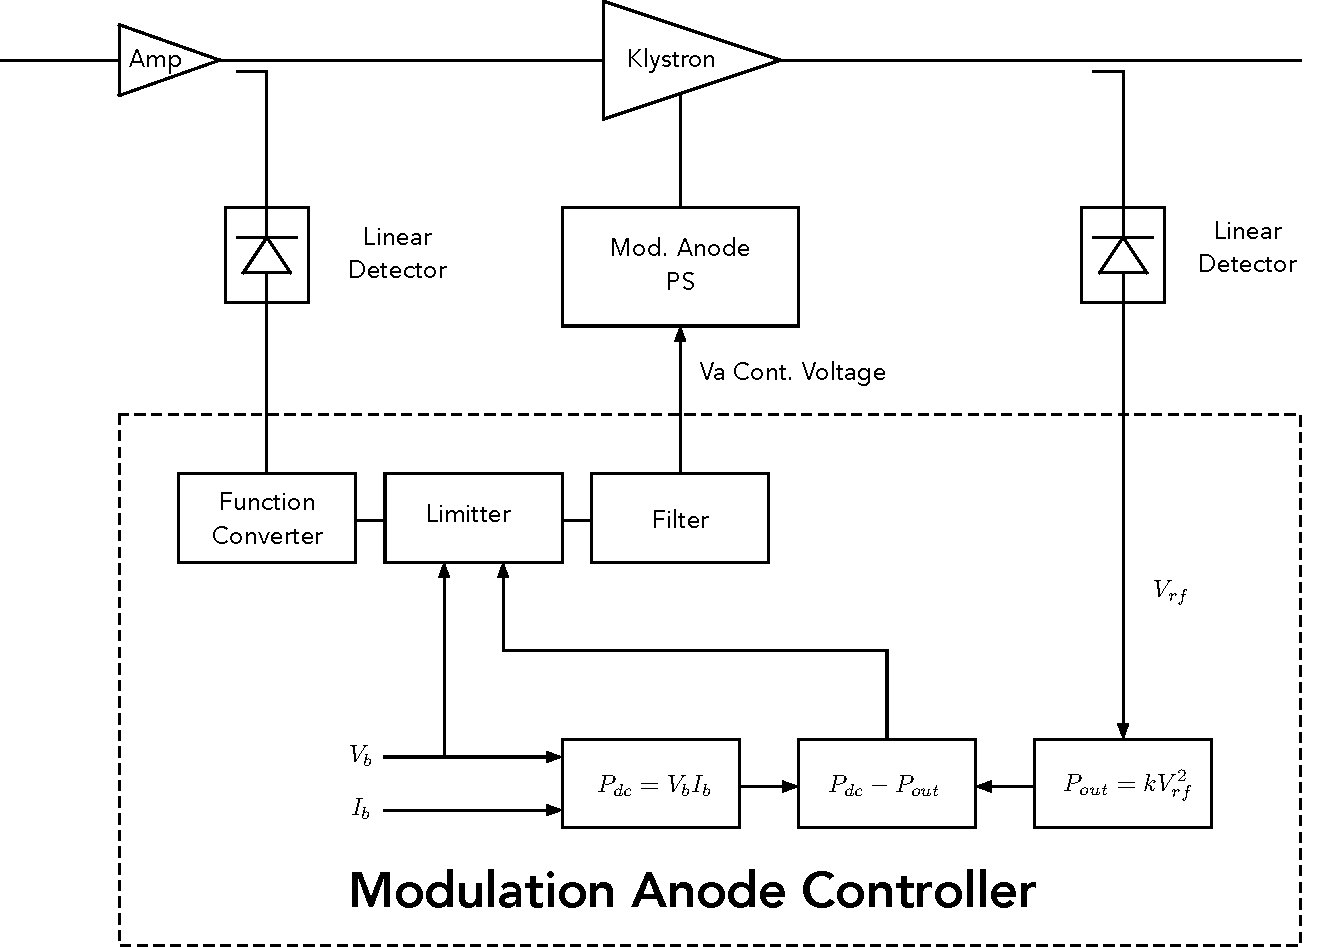
\includegraphics[width=\linewidth]{figs/Mod_Anode.pdf}
        \caption{Block diagram of the klystron beam-current control system.}
        \label{mod_anode}
    \end{center}
\end{figure}
%
\begin{figure}[hbt]
    \begin{center}
        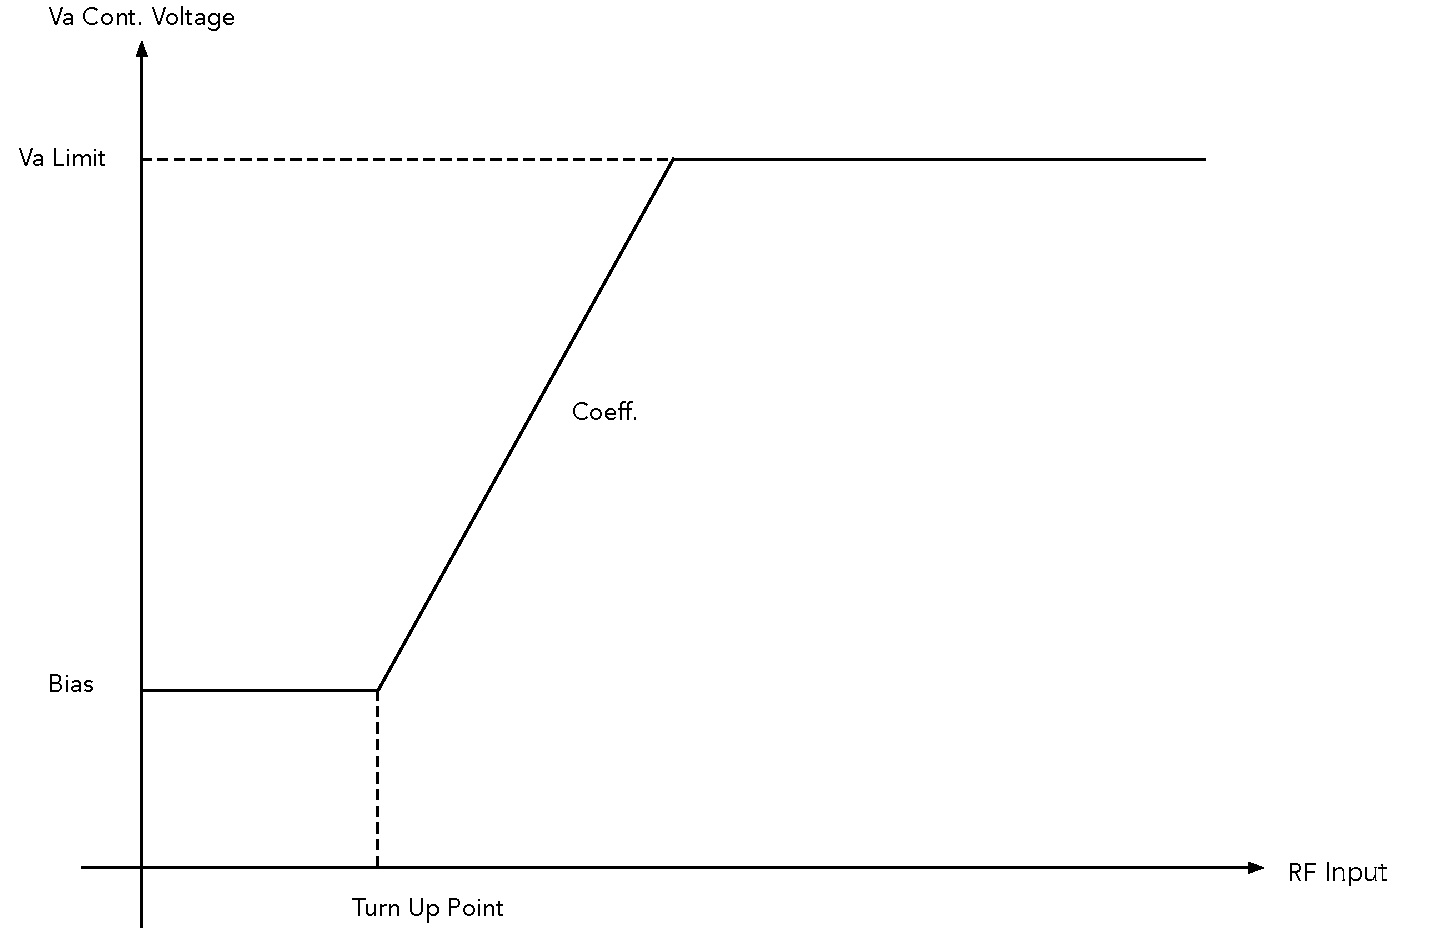
\includegraphics[width=\linewidth]{figs/Func_Conv.pdf}
        \caption{関数変換器の出力}
        \label{func_conv}
    \end{center}
\end{figure}

%
\end{document}